\documentclass{article}

\usepackage{fancyhdr}
\usepackage{ragged2e}
\usepackage{graphicx}
\usepackage{caption}
\usepackage{geometry}
\usepackage{amsmath}
\usepackage{rotating}

\usepackage{listings}
\usepackage{color}

\definecolor{dkgreen}{rgb}{0,0.6,0}
\definecolor{gray}{rgb}{0.5,0.5,0.5}
\definecolor{mauve}{rgb}{0.58,0,0.82}

\lstset{frame=tb,
  language=Java,
  aboveskip=3mm,
  belowskip=3mm,
  showstringspaces=false,
  columns=flexible,
  basicstyle={\small\ttfamily},
  numbers=none,
  numberstyle=\tiny\color{gray},
  keywordstyle=\color{blue},
  commentstyle=\color{dkgreen},
  stringstyle=\color{mauve},
  breaklines=true,
  breakatwhitespace=true,
  tabsize=4
}

\setcounter{secnumdepth}{1}

\usepackage{chngcntr}
\counterwithin{figure}{section}

\renewcommand*{\thepage}{C\arabic{page}}

\pagestyle{fancy}
\lhead{ACME Robotics}
\chead{\#8367}
\rhead{\ifcontents Contents \else Week \thesection \fi}

\newif\ifcontents
\contentstrue

\makeatletter
\renewcommand{\@seccntformat}[1]{}
\makeatother

\begin{document}\contentsfalse
\subsection{Decide what business tasks need to be completed before the Burlingame competition}
%! Create tasks in Jira that need to be executed before ACME's first competition.
With the team's first competition confirmed, Emma thought it might be good to start figuring out what business tasks needed to be completed before hand. Using the business Jira board, Emma wrote up tasks that covered all areas of the business team. Such as, finishing fundraising letters, writing up the goals and action plan in the EN, and writing up ACME's outreach events in the EN. Having a list of tasks written out, whether on paper or on a screen, is better way to keep track of tasks rather than just having a running list in your head. Most of the tasks she created were specific to the EN and need to be completed before their first tournament. She will be working on several of these tasks in the weeks to come.

\subsection{Finalize the budget with the team captains}
%! Decide on the final budget for the build.
Finalizing the budget for the season was important to complete sooner rather than later because so many other tasks (especially business tasks) depended on it. Using the list of parts needed for the robot, the team was able to estimate how much all of the parts would cost (\$2500), including how many extras they were going to need to build spare parts just in case something broke on the robot. The team also left enough room in the budget to allow for iteration, if need be (\$1500). That total came out to be \$2,200. As an extra precaution, the team decided to add about 30\% of wiggle room onto that total, bringing the total number to \$6000. The team thinks that this is a very reasonable number and is planning to reach it by sending out fundraising letters to the community. As the team is not supported by any school, it is important to decide the budget as early as possible in order to send them out quickly.

\subsection{Print, sign, address, stamp and send the fundraising letters}
%! Completely finish the process of sending out fundraising letters to sponsors.
Although the fundraising letters were already written, the team still needed to print them out, address them, and mail them. Emma printed out over 50 individually addressed letters. Then, she, Kelly, and Sean and Eli from ARES signed their names at the bottom of the letters. ACME believes that this looks professional and adds a bit of a personal touch to each letter.  Eli and Sean addressed each envelope and the mentors sent them out later that day, as you can see in figure \ref{fig:Letters}. Both teams are expecting funds to come in the coming weeks. 

\begin{figure}
    \centering
    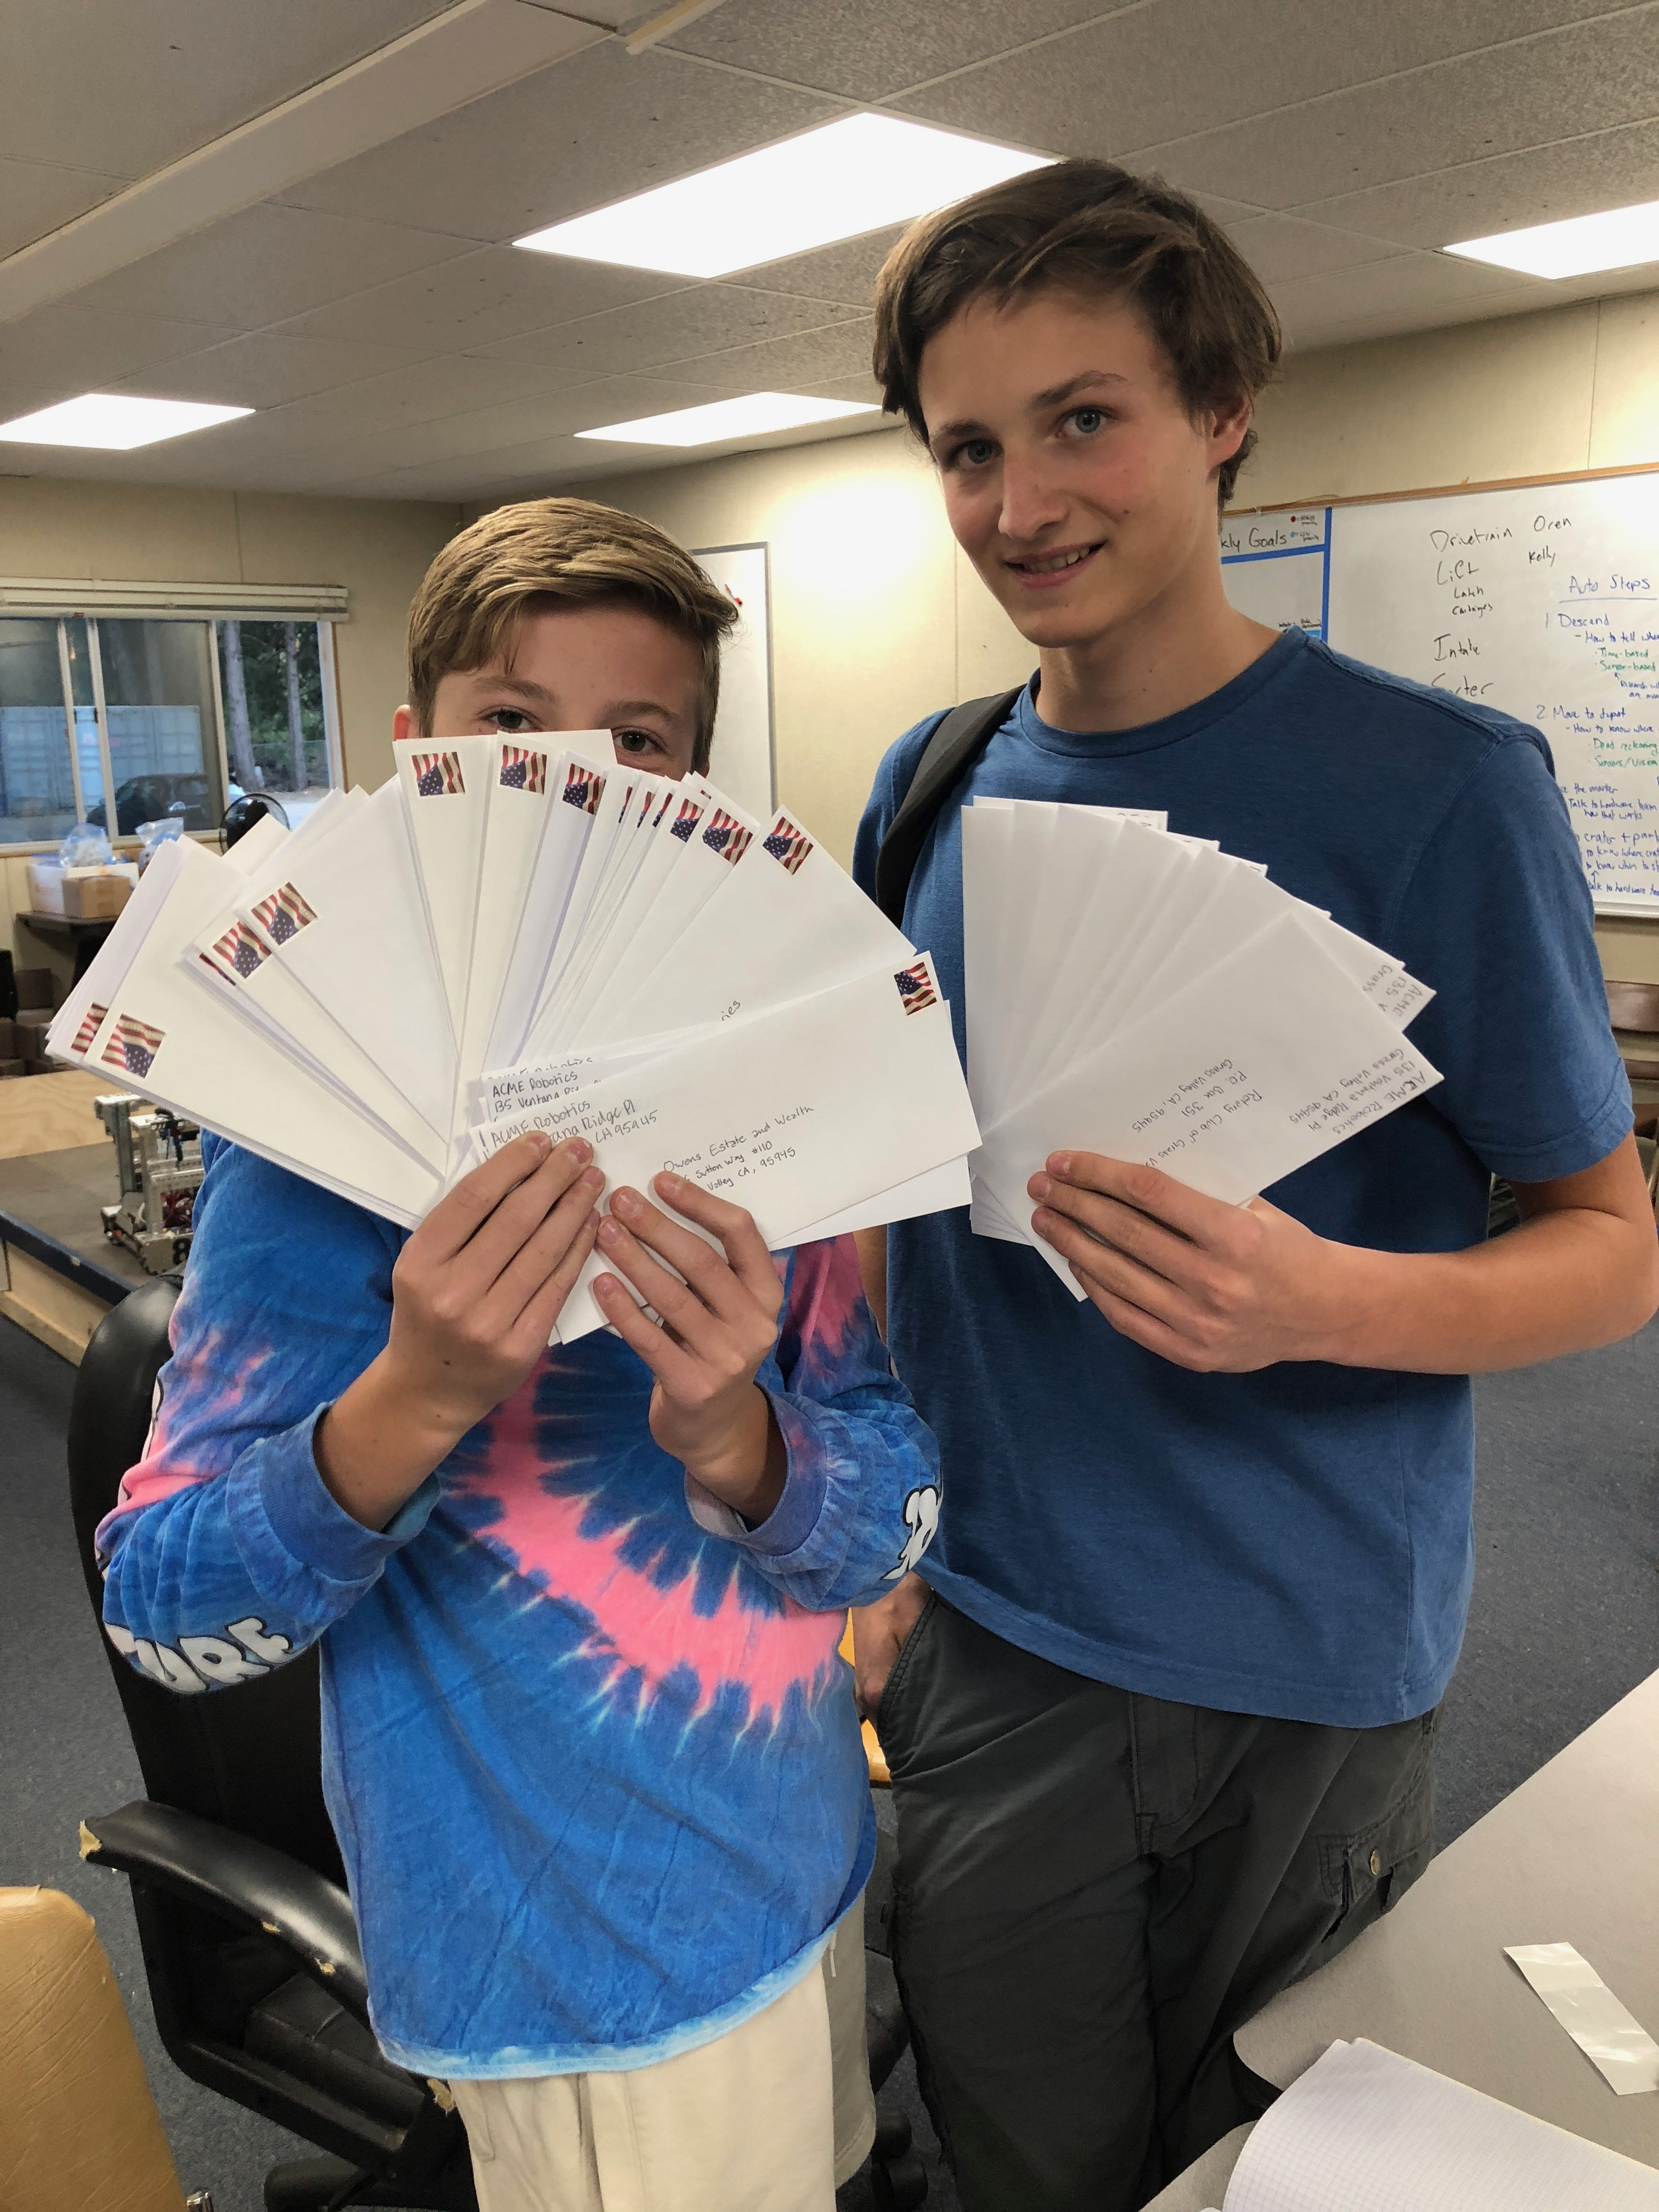
\includegraphics[width=.6 \textwidth]{07_10-15/images/letters.jpg}
    \caption{Eli and Sean with the final letters}
    \label{fig:Letters}
\end{figure}

\subsection{Start interviewing team members for bios}
%! Interview ACME members for their bios in the business notebook.
As always, the most distracting task of the season has come again. This is of course, interviewing members for their bios in the Business Notebook. Why is it so distracting to people? Because listening to Emma and Kelly give an interview to each member is for some reason very entertaining. Besides that they were able to gather all of the information that they needed. Some of the questions asked were, "What is your wildest idea for a FTC challenge?" and "What is your favorite gracious professionalism story?" Emma plans to type these bios up in \LaTeX along with a photo of each team member, as shirts and jackets arrive. 


\end{document}